\section{Case Study: Rössler System}

The well known Rössler system is given by the equations
\[
	\begin{array}{rcl}
		\dot x &=& -y - z \\
		\dot y &=& x + a \cdot y \\
		\dot z &=& b + z \cdot (x - c) \\
	\end{array}
\]
with parameters $a$, $b$, and $c$. For this example, $a$ and $b$
are fixed to $0.1$, while we are varying $c$.

The system has several periodic solutions for each value of $c$ with different
periodicities, though only one is stable at a time. We are interested in the origin and
branching of those solutions and, thus, drawing a bifurcation diagram using the map
\[
	f \mapsto \{ \|f(t)\|_2  \ | \ t \in [0, 2\pi), \ f(t)_1 = 0 \} \ .
\]
Here, $f$ denotes a single periodic solution. Note, that we use only the approximation
given by Galerkin's method.

Now, the exploration of the bifurcation with the given tools follows rougly this steps:
\begin{enumerate}
	\item As a starting point, search for a value of $c$ such that the system has a
		stable, periodic solution and use the method described in
		\autoref{sec:initial} to find it. 4000 iterations in the transient part with step
		size of $0.01$, 120 generated intersections with the $(x=0)$-plane and tests for
		at most $30$ periods were sufficient for all initial solutions of the Rössler
		system. We started at $c=4$ with $64$ samples.
	\item Trace out the branch just by following the newly found solution in both directions
		using the predictor-corrector continuation method (\autoref{sec:cont}). The
		parameters $\kappa=0.4$, $\delta=3.0$, and $\alpha=10.0$ are a decent choice for
		the whole diagram as a good tradeoff between performance and accuracy.
	\item It is possible to detect a pitchfork bifurcation by doubling up the periodicity
		artifically. Using the described predictor-corrector method, the value
		of $c$ will eventually converge to the bifurcation point, i.e., a point with a
		singular tangent. Since the method is now stuck, reaching the doubly-periodic
		solution can be done by solving a slightly perturbed problem for a short time.
		A short perturbation of strength $0.2$ was enough to reach the doubly-periodic
		solution. Also, it might be necessary to increase the sample size due to increased
		complexity in the descending branch.
	\item Remove the perturbation and continue tracing out the bifurcation, i.e. start
		over in 1 or 2.
\end{enumerate}

\begin{figure}[!ht]
	\centering
	\subfloat[][]{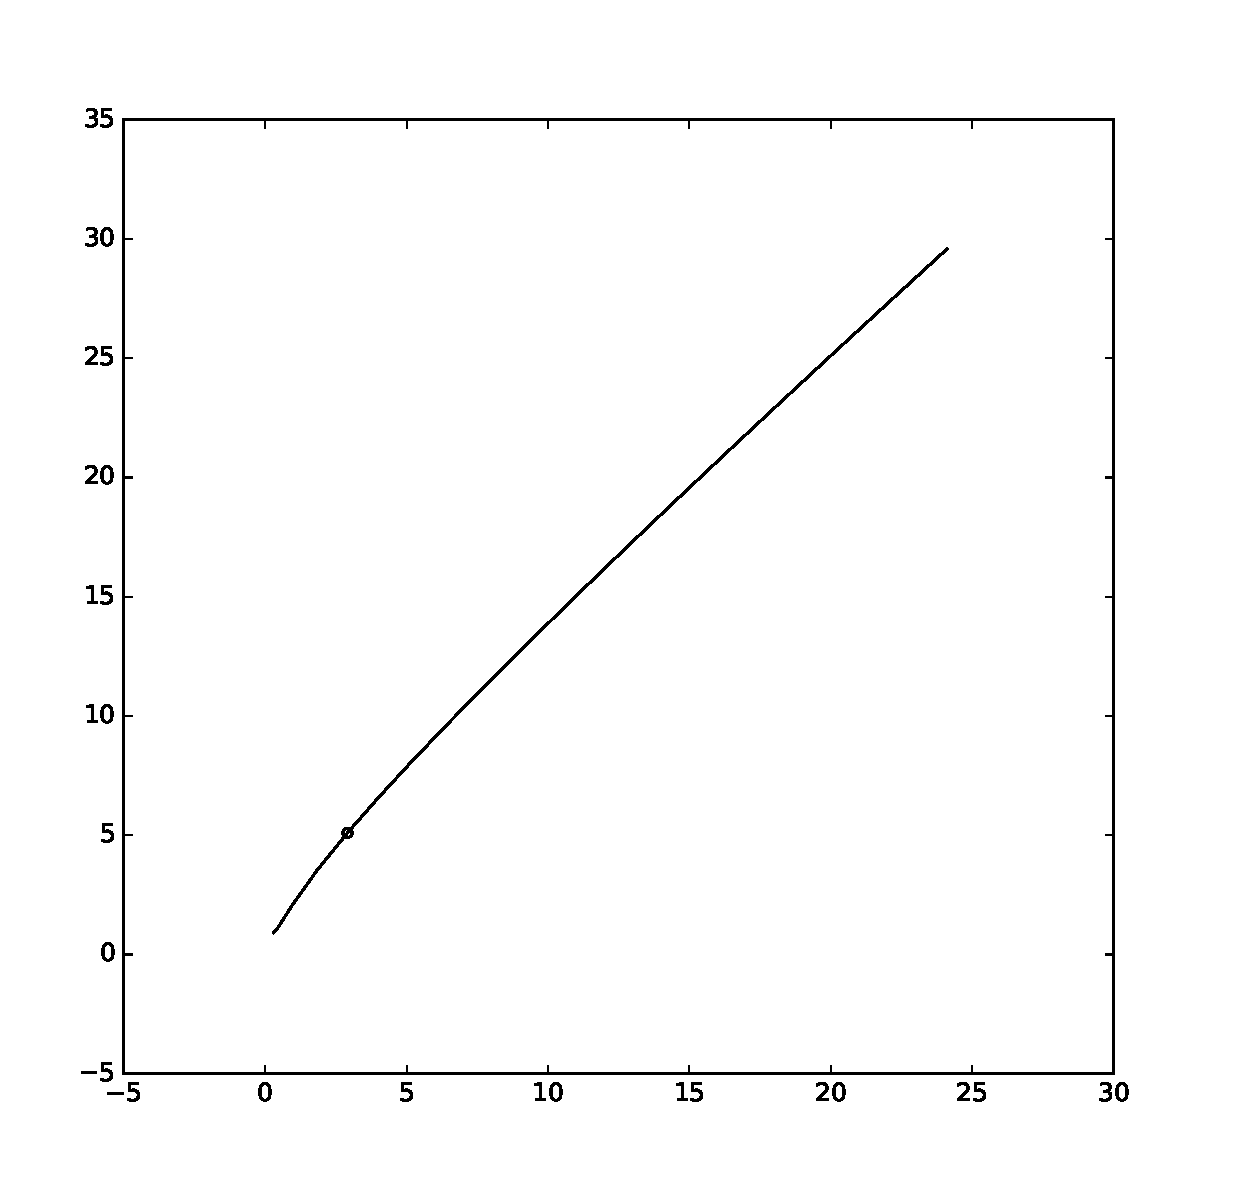
\includegraphics[width=.4\textwidth]{img/roessler1a.pdf}}\quad
	\subfloat[][]{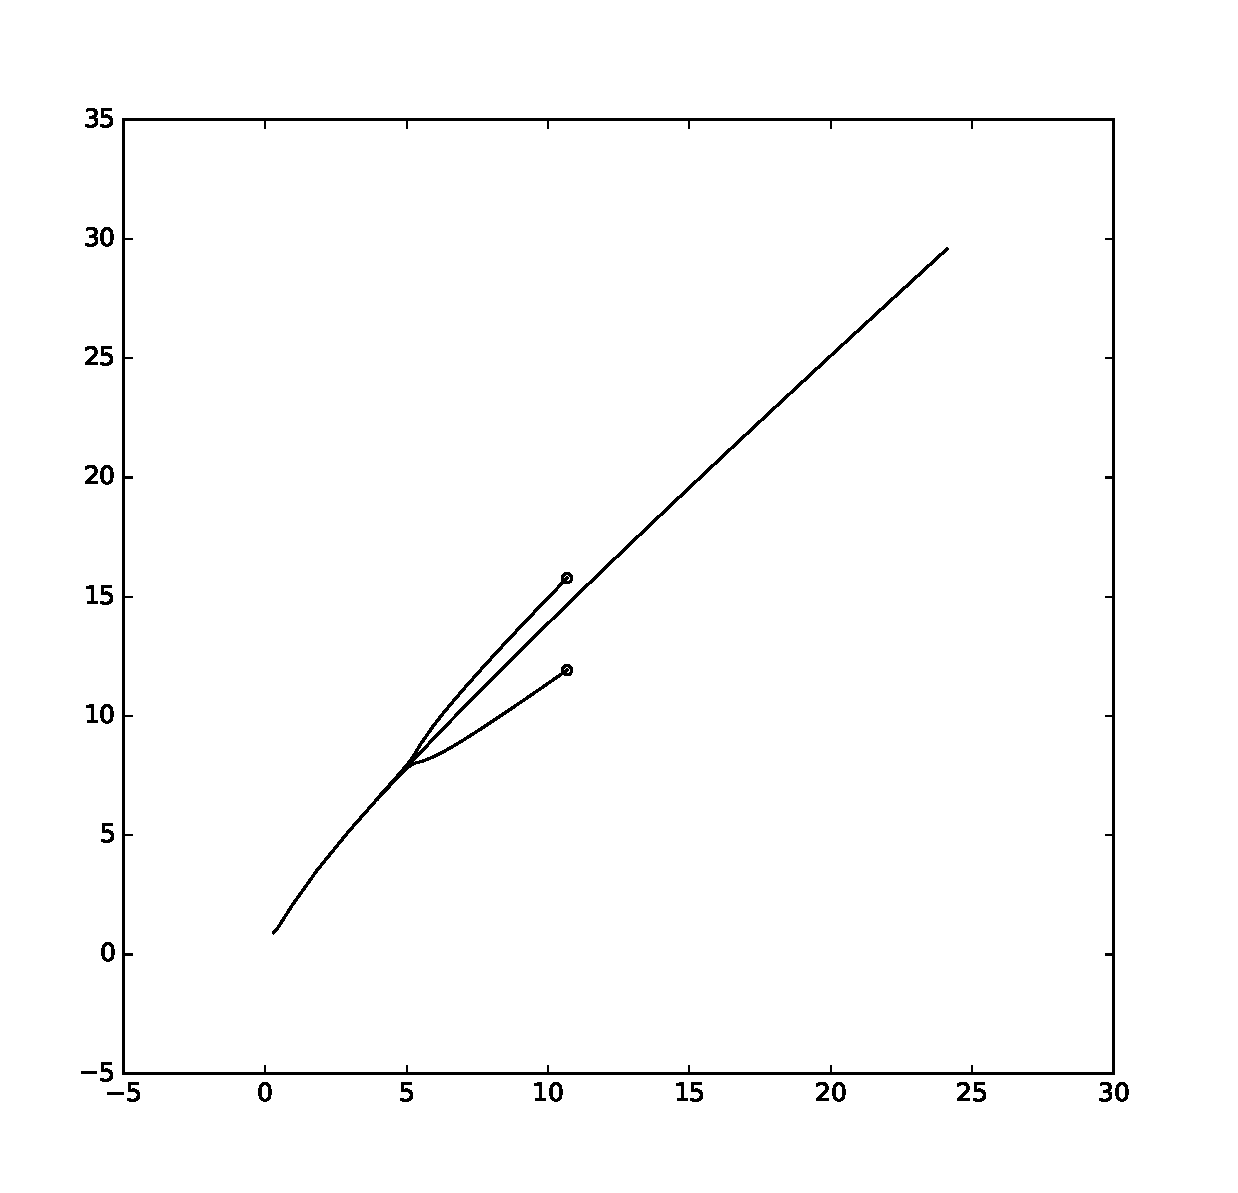
\includegraphics[width=.4\textwidth]{img/roessler1b.pdf}}\\
	\subfloat[][]{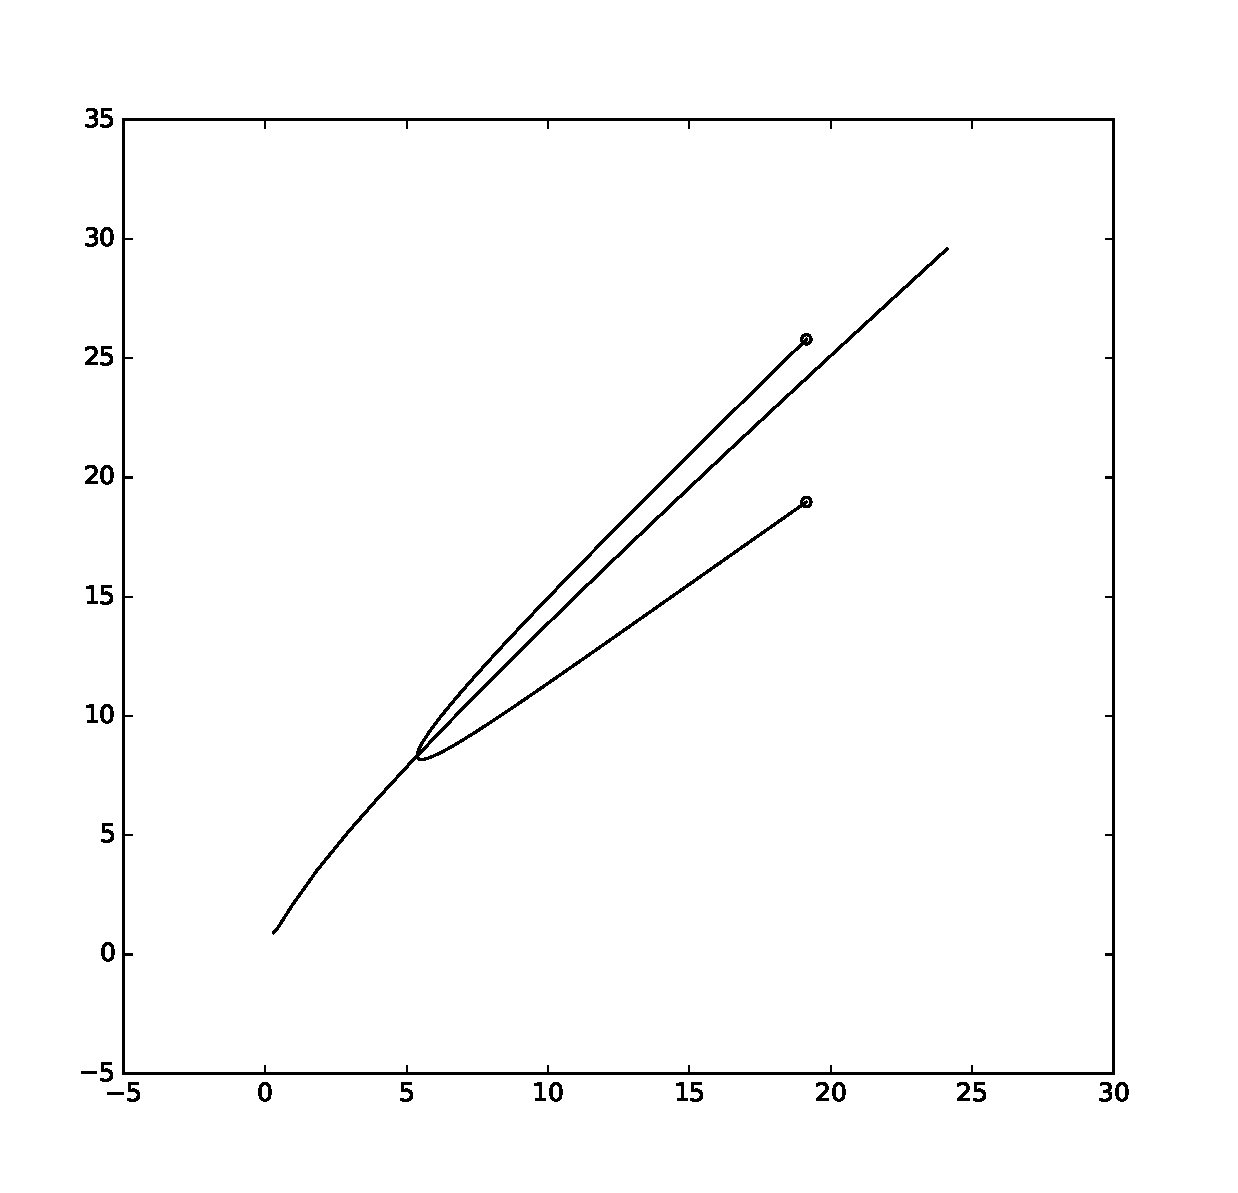
\includegraphics[width=.4\textwidth]{img/roessler1c.pdf}}\quad
	\subfloat[][]{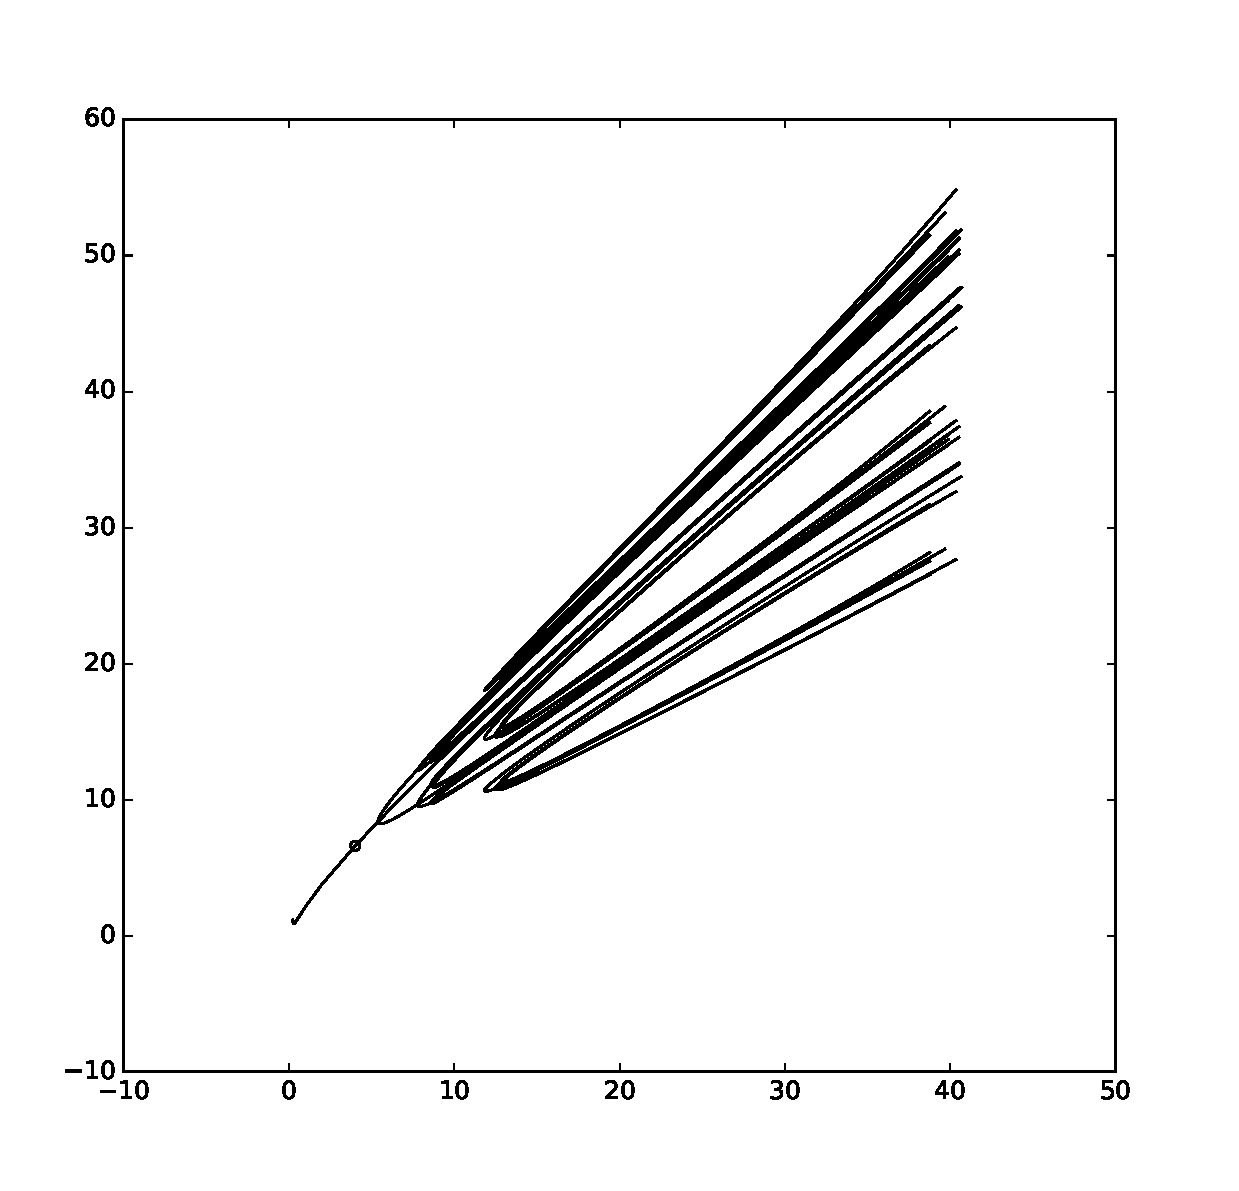
\includegraphics[width=.4\textwidth]{img/roessler1d.pdf}}
	\caption{Tracing out the branch of solutions beginning with the solution for
	$c=4$ (a). The bifurcation point in $c \approx 5.376$ is avoided by using a permutation (b),
	and the two-periodic solutions can be traced out after removing the inaccurate values
	from before (c). Eventually, we reach (d), a widely traced out bifurcation diagram.
	Note the solutions with periodicity three and descendants, that do not originate in
	the peridocity-one branch.}
	\label{fig:sub1}
\end{figure}

\begin{figure}[!ht]
	\centering
	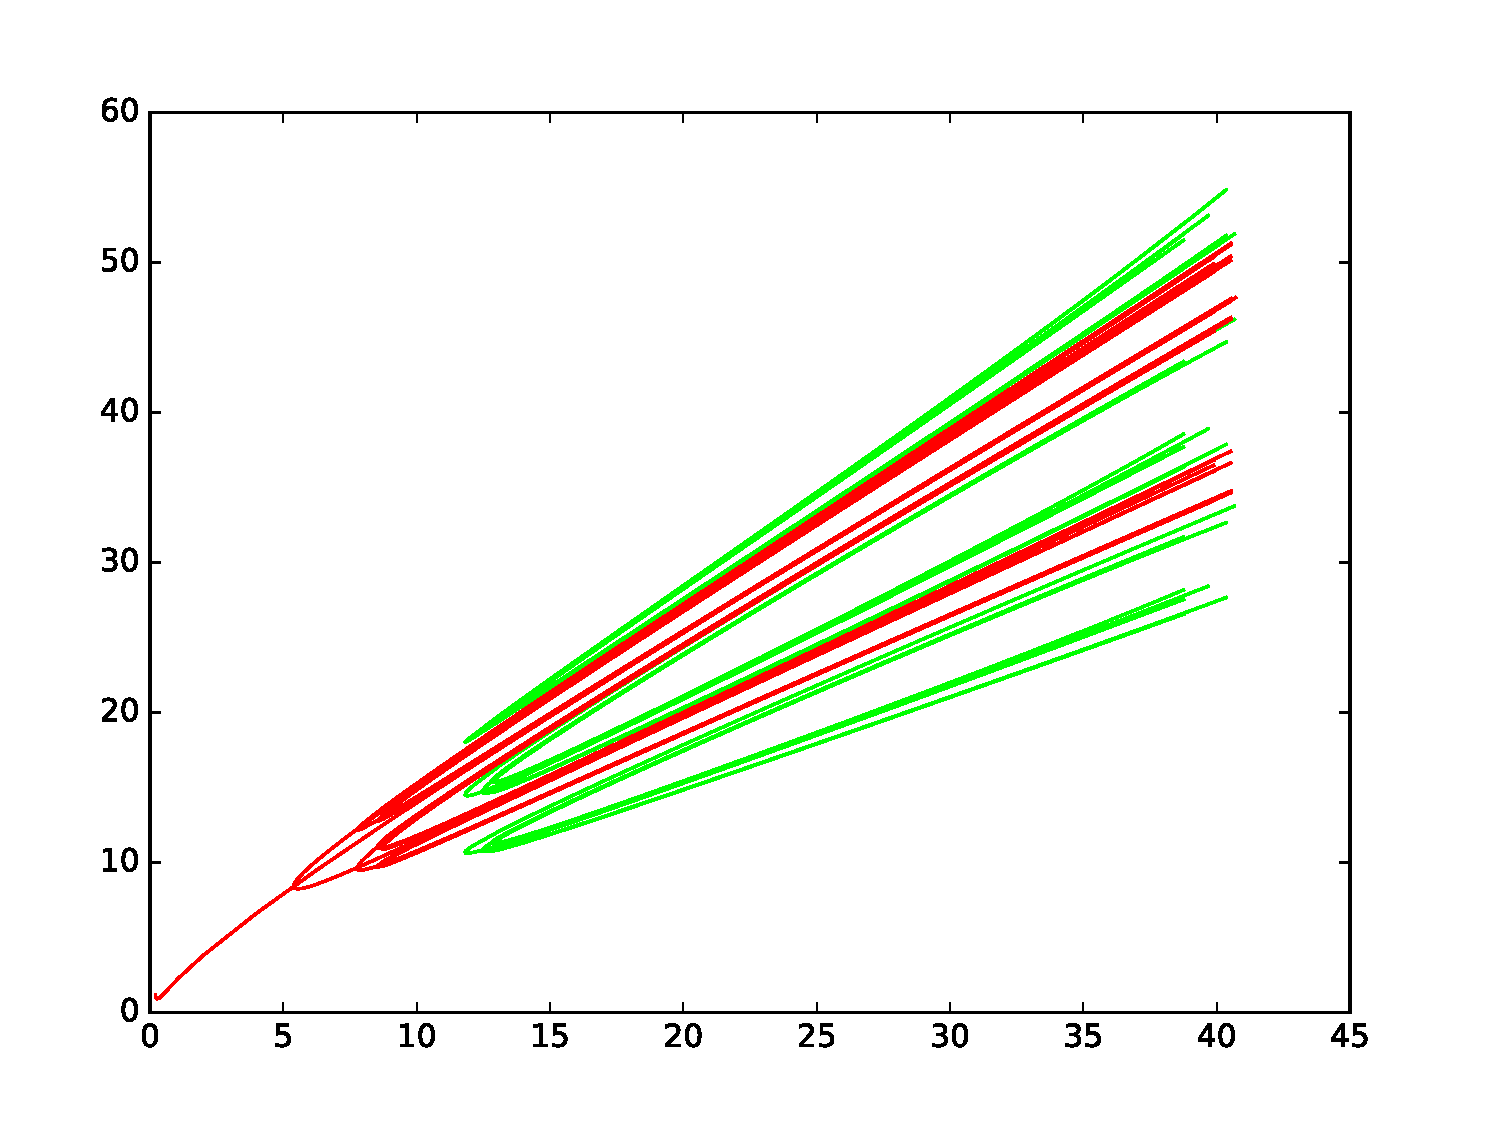
\includegraphics[width=1\textwidth]{img/roessler2a.pdf}
	\caption{The bifurcation diagram of the Rössler system for varying $c$. The
		even-periodic solutions are colored red, the odd-periodic ones green.}
\end{figure}

\begin{figure}[!ht]
	\centering
	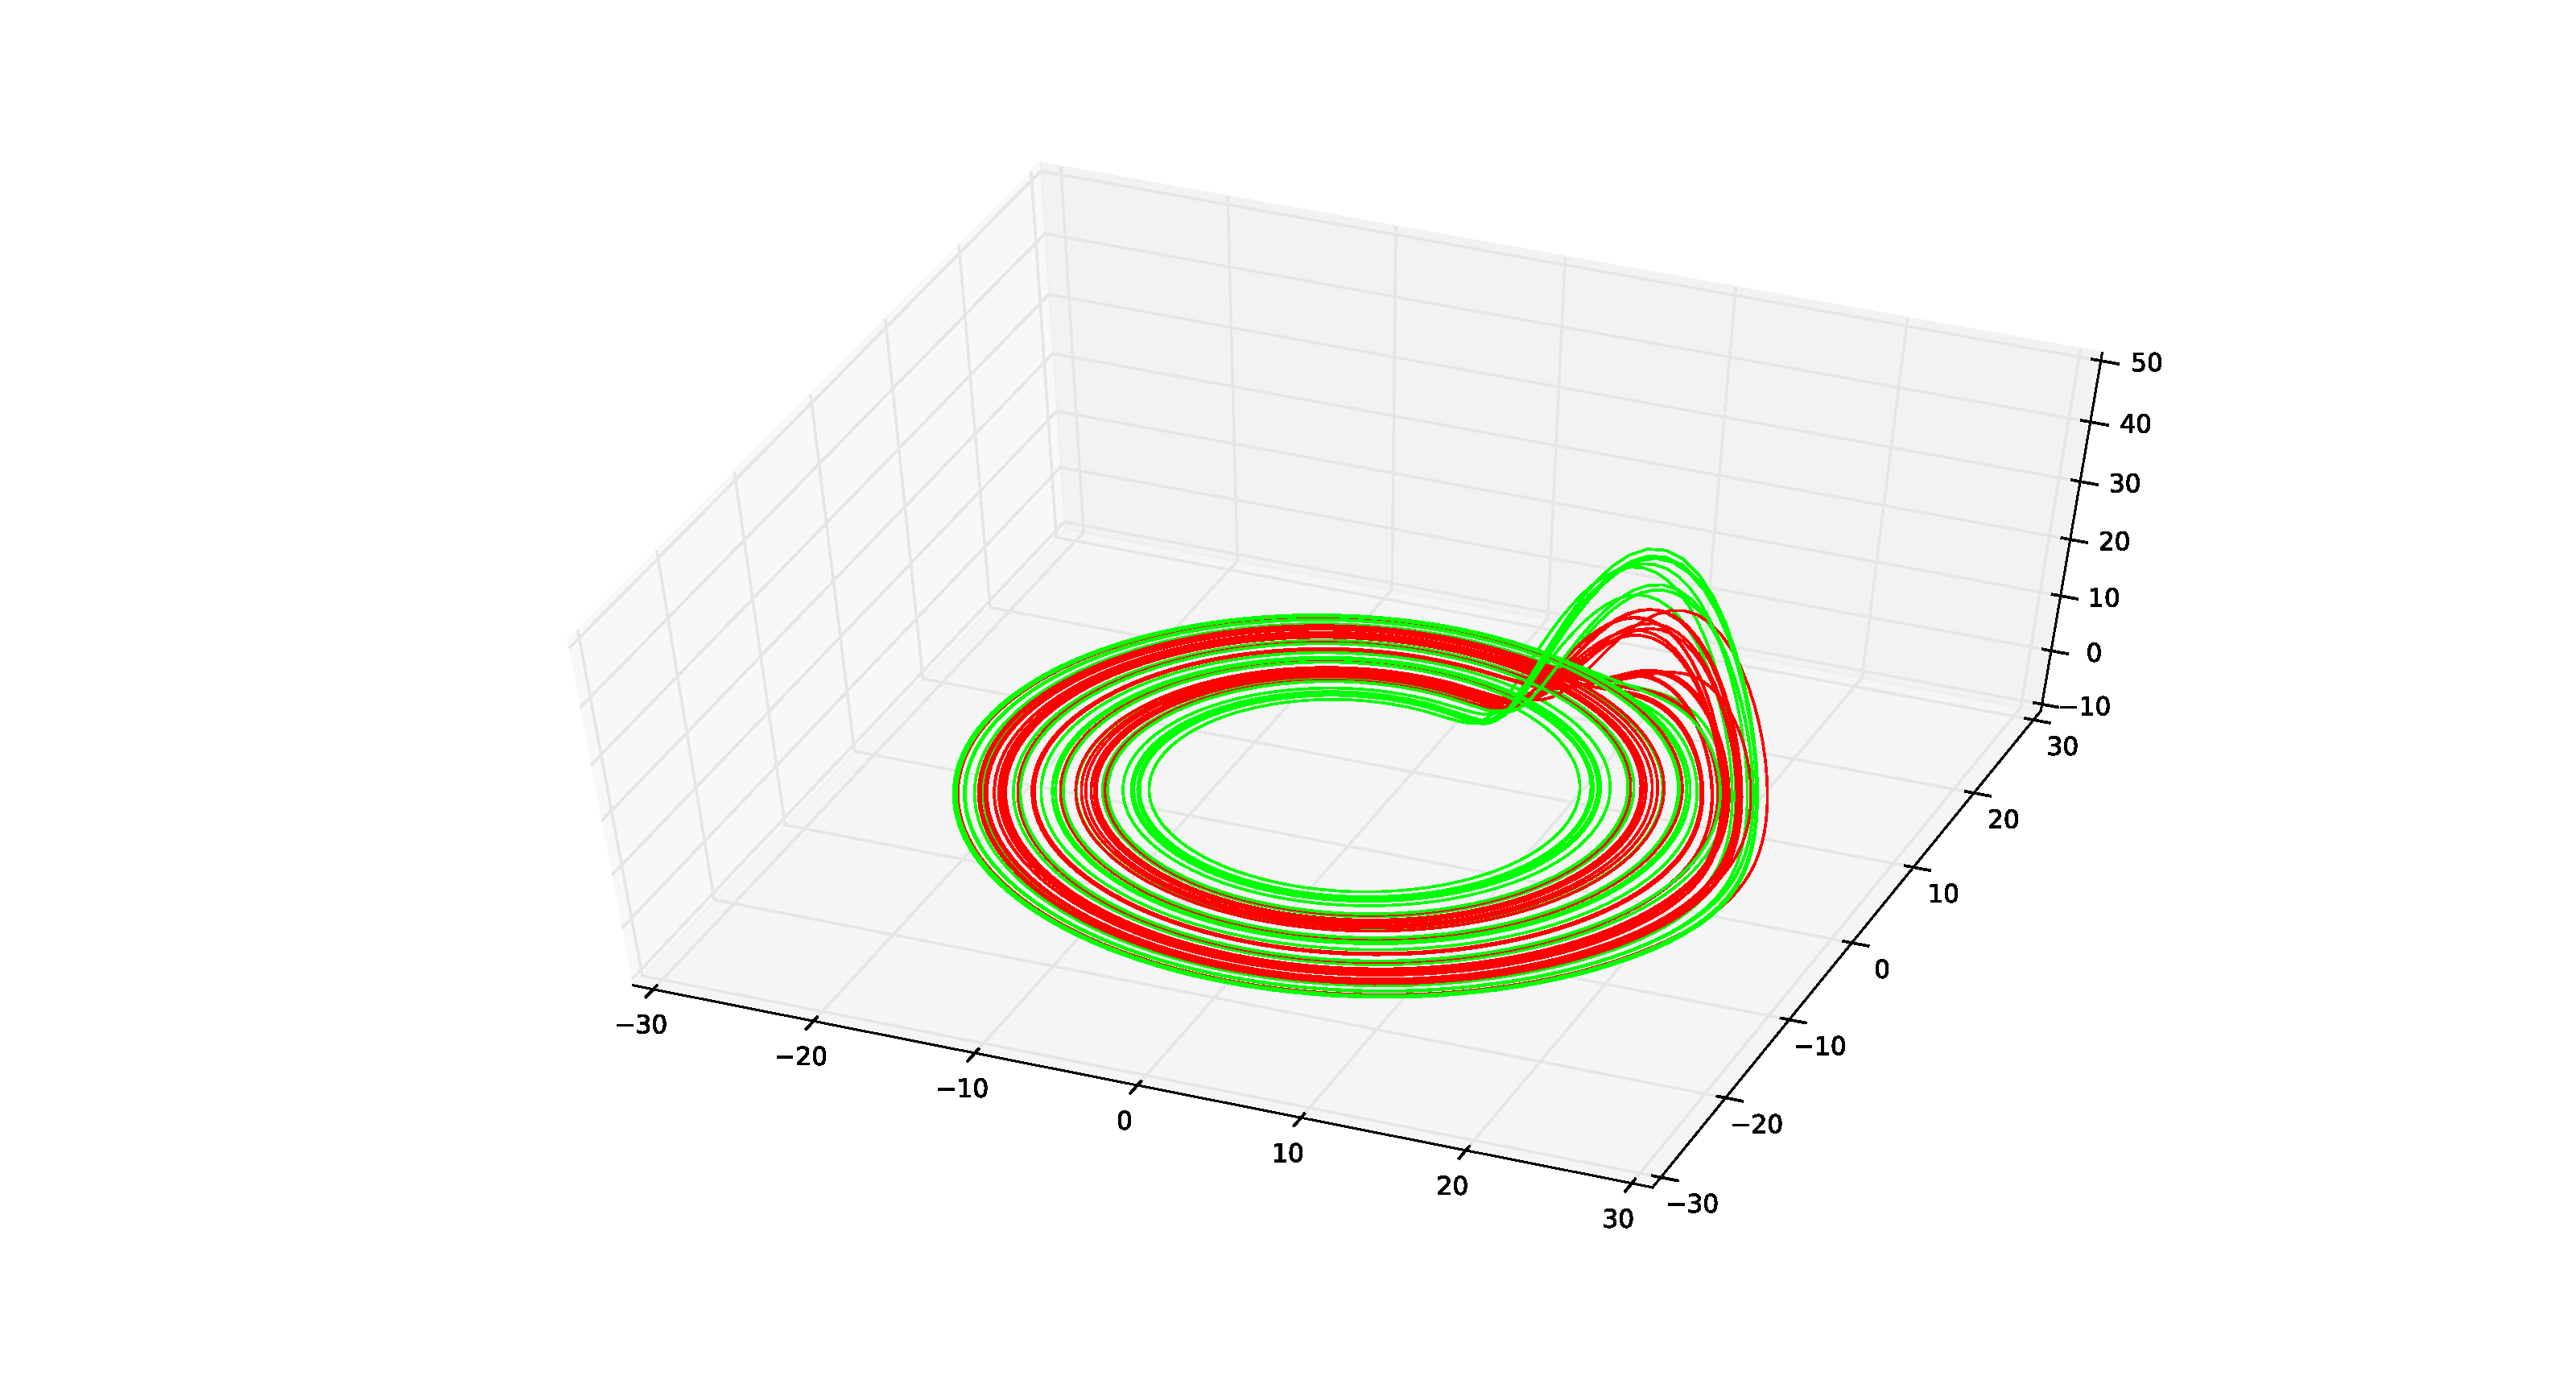
\includegraphics[width=1\textwidth]{img/roessler2b.pdf}
	\caption{All found solutions for $c=\dots$ plotted into one diagram.
	Observe how the odd-periodic and even-periodic solutions dodge since they do not
	originate from each other.}
\end{figure}



